\documentclass[a4paper,12pt]{article}
\usepackage[english]{babel}
\usepackage{graphicx}
\usepackage{tikz}
\usepackage{wrapfig}
\usepackage{array}
\usepackage{color} 
\usepackage{hyperref}
\usepackage{enumitem}
\usepackage[font=small,labelfont=bf]{caption}
\hypersetup{
    colorlinks,
    citecolor=black,
    filecolor=black,
    linkcolor=black,
    urlcolor=black
}
\usepackage{changepage}
\addto{\captionsenglish}{\renewcommand{\refname}{}}

\begin{document}

\title{%
  Group Project Part 1 - Neo4j \\
  \large of Systems and Methods for Big
    and Unstructured Data Course \\(SMBUD)\\
    held by\\ Brambilla Marco\\ Tocchetti Andrea \\
  \vspace{5mm}
  \Large \textbf{Group 14}}
\author{Banfi Federico\\
  \texttt{10581441}
  \and
  Carotenuto Alessandro\\
  \texttt{10803080}
  \and
  Donati Riccardo\\
  \texttt{10669618}
  \and
  Mornatta Davide\\
  \texttt{10657647}
  \and
  Zancani Lea\\
  \texttt{10608972}}
\date{Academic year 2021/2022}
\maketitle
\begin{center}
  \includegraphics[width=4cm]{polilogo.png}\\
\end{center}
\newpage
\tableofcontents
\newpage
\section{Problem Specification}
\paragraph{}The sanitary emergency caused by the spread of the SARS-CoV-2 virus and the pandemic that has spread since 2019 has highlighted how the Big Data and the applications based on the large-scale use of these technologies can lead to concrete and effective results in a short time. Among the main examples that can be cited with regard to these there is the contact tracing, i.e. the process of attempting to identify people who have recently been in contact with someone diagnosed with an infectious disease, especially in order to treat or quarantine them. \par
The purpose of our group project is to build an information system that allows us to manage pandemic information for a given country. In order to do this we have to design, store and query a graph data structure in a NoSQL DB, by means of the graph database management software Neo4j, supporting a contact tracing app for COVID-19.
\section{Hypotesis}
\paragraph{} The way in which the database was structured and implemented is based on some hypotheses discussed in the design phase. \par Considering a typical scenario in which each person can interact either with people who live with him (family members or roommates) or with other people who go to meet voluntarily or not in a limited closed place (for example a gym, a public place, a restaurant, etc.) or in an open place located in a generic position, it was assumed that the infection can occur if during the contact between the two subjects (one of which is potentially infected) the distance between them was particularly close and if the contact duration was at least 15 minutes. In addition, to check the state of health of each individual in relation to the pandemic situation, it is essential to consider whether they have been given a vaccine and/or whether they have recently undergone a test to check for any positivity. \par
Specifically, in order to simulate the pandemic situation in the most realistic way possible and to optimally manage the available data that an information system directly connected to an app supported by the database will have to process, the following assumptions were taken into consideration:
  \begin{enumerate}[noitemsep]
    \item people can go to public places even without a green pass (therefore without a vaccine or a negative test carried out in the last 48 hours),
    \item data relating to public places are sent to the system by the manager of the public place itself,
    \item to record a greater number of relationships to be processed, while ensuring the consistency and meaningfulness of the stored data, it was decided to limit to an example study case in which the interactions present in the dataset are related to the single city of Milan and for a limited time interval, therefore:
  \begin{itemize}[noitemsep]
    \item[-] the tests dates, the meetings between people and the visits to public places took place from the 15\textsuperscript{th} of October to the 15\textsuperscript{th} of November, in addition, to test the queries more easily, there is a specific date, i.e. the 31\textsuperscript{st} of October, that expressely presents multiple recorded interactions,
    \item[-] vaccine administrations were all performed within the last year,
    \item[-] all public places are located in Milan,
    \item[-] meetings between people are geolocated within the city limits
  \end{itemize}
    \item with regard to the various connections that can exist between several people and the infections that can occur within the same family, it was preferred, for design purposes, to consider the concept of "same residential unit" (i.e. residence) rather than that of "family", since belonging to a given family unit does not necessarily imply a constant coexistence (e.g. workers who often travel for a job or off-site students) while a relationship of coexistence between several people, not necessarily related to each other, usually involves a close and inevitable contact,
    \item concerning to meetings between two or more people, it was assumed that any contact tracing devices/ apps interact with the system, communicating this information for each meeting: person1, person2, time at which the contact took place, geographical point in where the contact took place,
    \item a person is considered infected from the moment he undergoes a test and receives a positive result until he takes another test again but it is negative,
    \item in the event that a person undergoes a test and receives a positive result, all people met in the 15 days prior to the test will receive an alert notification on the app ensuring the privacy of the infected person is safeguarded,
    \item the possibility has also been envisaged in which a person already vaccinated may still be infected, in line with the cases that actually occurred
  \end{enumerate}
\clearpage
\section{ER diagram}
\paragraph{}
	\begin{center}
 		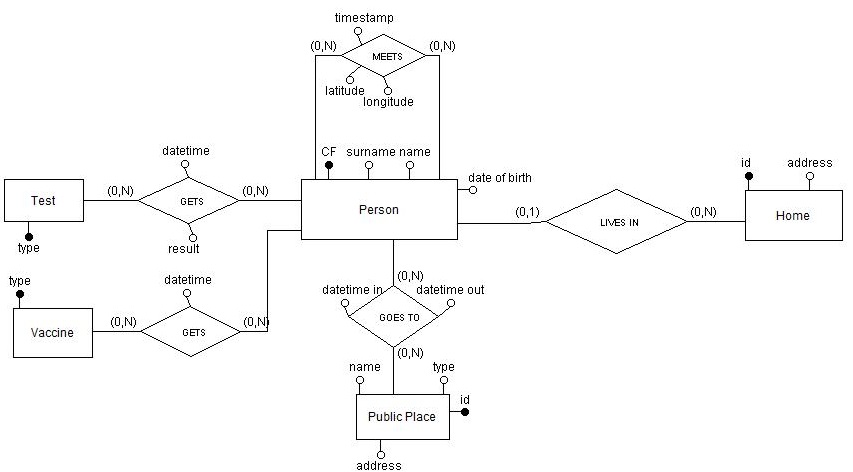
\includegraphics[width = 15 cm]{ER_diagram.jpg}
		\captionof{figure}{E-R Diagram}
	\end{center}
\par Starting from the considerations previously exposed regarding the implementation hypotheses, we have drawn an ER diagram (\textbf{Figure 1}) which includes 5 different entities and 4 many-to-many relationships described below in the logical model: \par
  \begin{itemize}[noitemsep]
   	\item[-]	\textbf{Person}(\underline{CF}, Name, Surname, DateOfBirth)
	\item[-]	\textbf{Vaccine}\underline{(Type})
	\item[-]	\textbf{Test}(\underline{Type})
	\item[-]	\textbf{PublicPlace}(\underline{ID}, Name, Type, Address)
	\item[-]	\textbf{Home}(\underline{ID}, Address)
	\item[-]	\textbf{Met}(\underline{Person.CF}, \underline{Person.CF}, Latitude, Longitude, Timestamp)
	\item[-]	\textbf{GotTested}(\underline{Person.CF}, \underline{Test.Type}, Datetime, Result)
	\item[-]	\textbf{Got}(\underline{Person.CF}, \underline{Vaccine.Type}, Datetime)
	\item[-]	\textbf{WentTo}(\underline{Person.CF}, \underline{PublicPlace.ID}, DatetimeIn, DatetimeOut)
  \end{itemize} \par
The \textbf{Person} entity describes every possible individual with his own personal data, the \textbf{Got} and \textbf{GotTested} relationships concern the Covid-related information of each one by means of \textbf{Test} and \textbf{Vaccine} that represent the actual types of vaccines and tests currently used. The \textbf{LivesIn} relationship allow us to keep track of all the people who share the same housing unit specified by the \textbf{Home}, while with \textbf{WentTo} it is possible to check who was in a specific place identified by \textbf{PublicPlace} through an address from a certain time until it went out. Finally, the \textbf{Met} relationship is used to keep track of all the people that everyone can meet during the day by recording with whom the meeting took place, when and where based on geographical coordinates, storing data only if the meeting duration was at least 15 minutes accordingly with the hypotheses specified before.
\section{Dataset description}
\paragraph{} One of the most critical parts of working with Big Data is managing large amounts of data collected in large datasets. To test and simulate the use of the database for contact tracing activities, some sample datasets were generated, saved in .csv format and imported into Neo4j through the command: \texttt{LOAD CSV FROM "file: ///file.csv" AS ...}. \par
Each dataset is divided into various fields that trace the structure of the tables expressed in the ER model, each one was generated randomly through Python scripts (you can find these ones into the folder \texttt{"db"}) and to experiment and perform at best the possible tests on the queries and commands that can be executed thanks to Neo4j the number of entries foreseen for each dataset is in the order of magnitude of the hundreds, as a whole, starting exclusively from the data loaded from the datasets, the database provides:
\begin{center}
\begin{tabular}{|l|l|l|l|}
\hline
Homes & 101 & Residence Relationship & 300 \\
\hline
People & 300 & Meetings & 726 \\
\hline
Public Places & 20 & Public Places Visits & 600 \\
\hline
Vaccine Types & 4 & Vaccinations & 526 \\
\hline
Test Types & 2 & Tests & 450\\
\hline
\textbf{TOTAL NODES} & \textbf{427} & \textbf{TOTAL RELATIONSHIPS} & \textbf{2602}\\
\hline
\end{tabular}
\end{center}
\section{Queries and Commands}
\paragraph{} The correct functioning of the information system involves the implementation of some essential commands and queries for the database in order to properly support the app and to ensure the right execution of searches among the data available for statistical or practical purposes. \par
\paragraph{} First of all you need to load the .csv files with the query you can find following the path \texttt{"documents/importDB.txt"}
\subsection{Queries}
\subsubsection{Find how many people went without greenpass in a public place}
\paragraph{} This query allows us to find all the people that went in a public place without the GreenPass and the datetime related.
\begin{center}
	\fbox{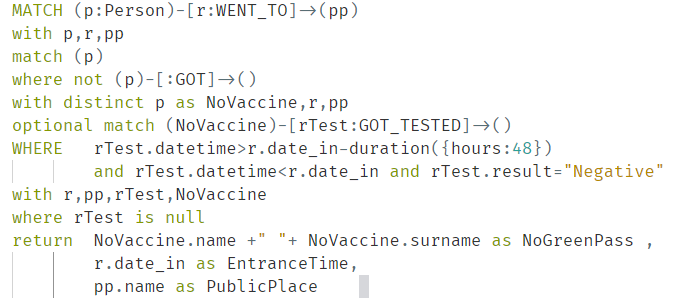
\includegraphics[width = 13 cm]{query1.png}}
\end{center}
\paragraph{} The output is given by: 
\begin{itemize}
\item[•] The name and the surname of the person
\item[•] The entrance time in the public place
\item[•] The name of the public place
\begin{center}
	\fbox{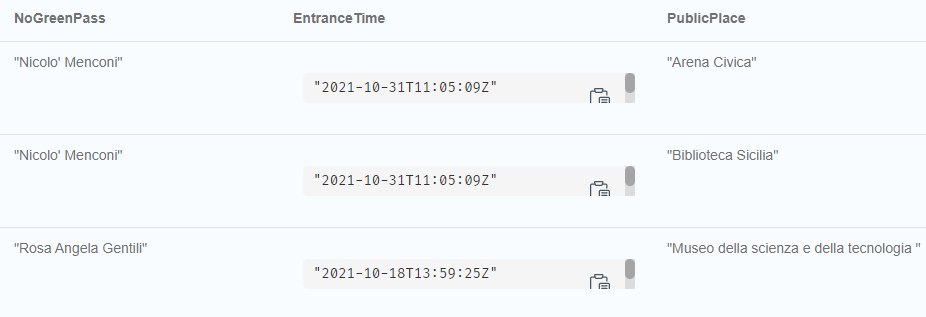
\includegraphics[width = 12 cm]{outputquery11.png}}
\end{center}
\end{itemize}
\clearpage
\subsubsection{Find who lives with an infected individual}
\paragraph{} This query allows us to detect a "family contact" with an infected person and obtain the people that need to be quarantined.
\begin{center}
	\fbox{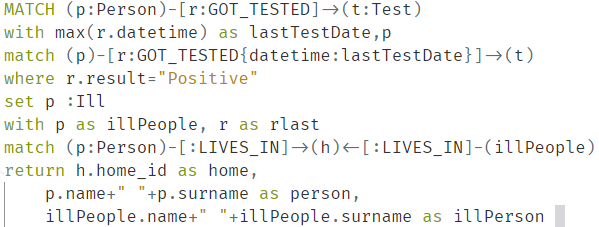
\includegraphics[width = 13 cm]{query2.png}}
\end{center}
\paragraph{} The output is given by: 
\begin{itemize}
\item[•] The house identifier
\item[•] The name and the surname of the person
\item[•] The name and the surname of the infected cohabitant
\begin{center}
	\fbox{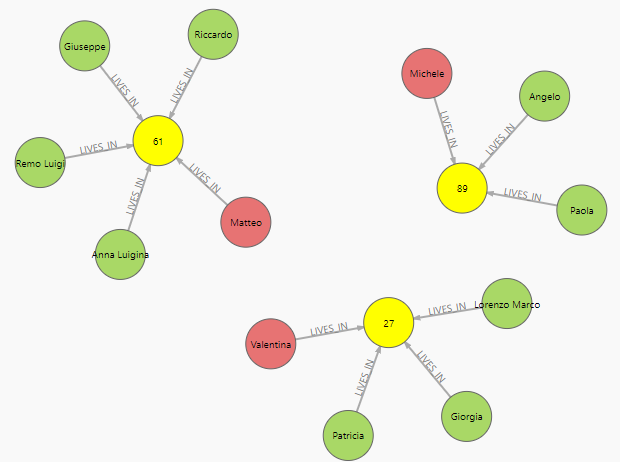
\includegraphics[width = 10 cm]{outputquery2.png}}
	\captionof{figure}{Visual representation of the result with NeoDash}
\end{center}
\end{itemize}
\subsubsection{Find public place contact with infect people}
\paragraph{} This query allows us to find the people who went in the same public place (e.g. restaurant, cinema,...) at the same time with infected people starting from 15 days before their positive test.
\begin{center}
	\fbox{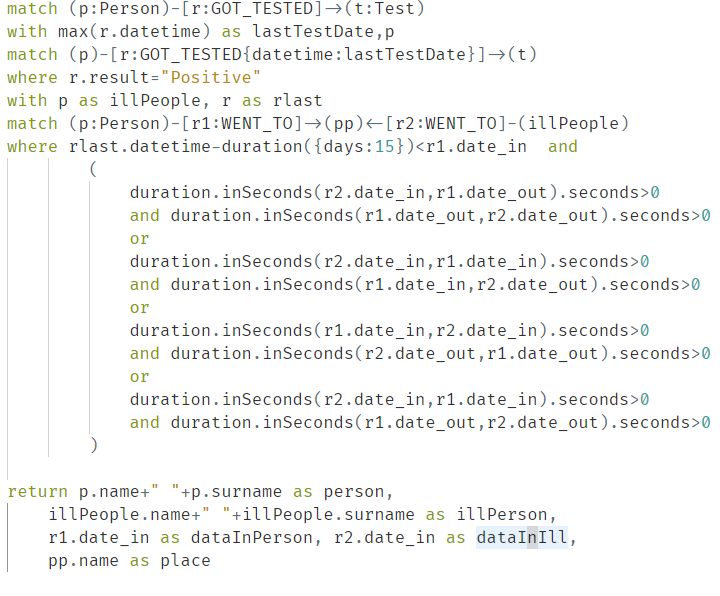
\includegraphics[width = 13 cm]{query3.png}}
\end{center}
\paragraph{} The output is given by: 
\begin{itemize}
\item[•] The name and the surname of the person
\item[•] The name and the surname of the infected cohabitant
\item[•] The datetime of the entrance of the health person
\item[•] The datetime of the entrance of the ill person
\item[•] The public place
\begin{center}
	\fbox{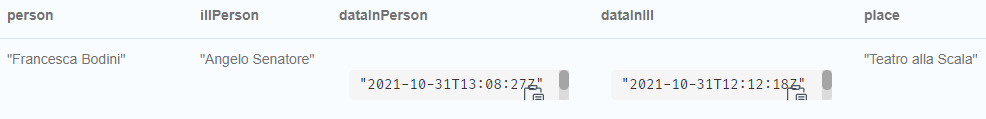
\includegraphics[width = 14 cm]{outputquery3.png}}
\end{center}
\end{itemize}

\subsubsection{Find who got vaccinated in a temporal range}
\paragraph{} This query allows us to find all the vaccinated people in the temporal range of October 2021.
\begin{center}
	\fbox{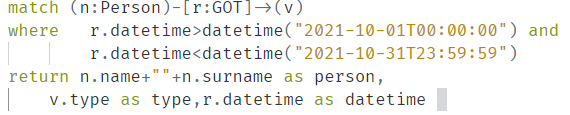
\includegraphics[width = 13 cm]{query4.png}}
\end{center}
\paragraph{} The output is given by: 
\begin{itemize}
\item[•] The name and the surname of the person
\item[•] The type of the vaccine
\item[•] The datetime of the vaccine
\begin{center}
	\fbox{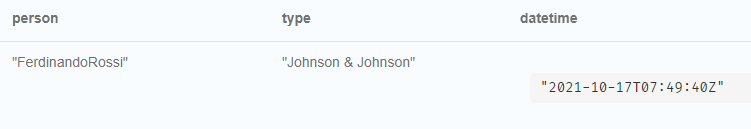
\includegraphics[width = 12 cm]{outputquery4.png}}
\end{center}
\end{itemize}
\pagebreak

\subsubsection{Statistical analysis of the vaccination campaign}
\paragraph{} This query allows us to compute an analysis on the number of the vaccinated people (and the percentage) grouped by age ranges.
\begin{center}
	\fbox{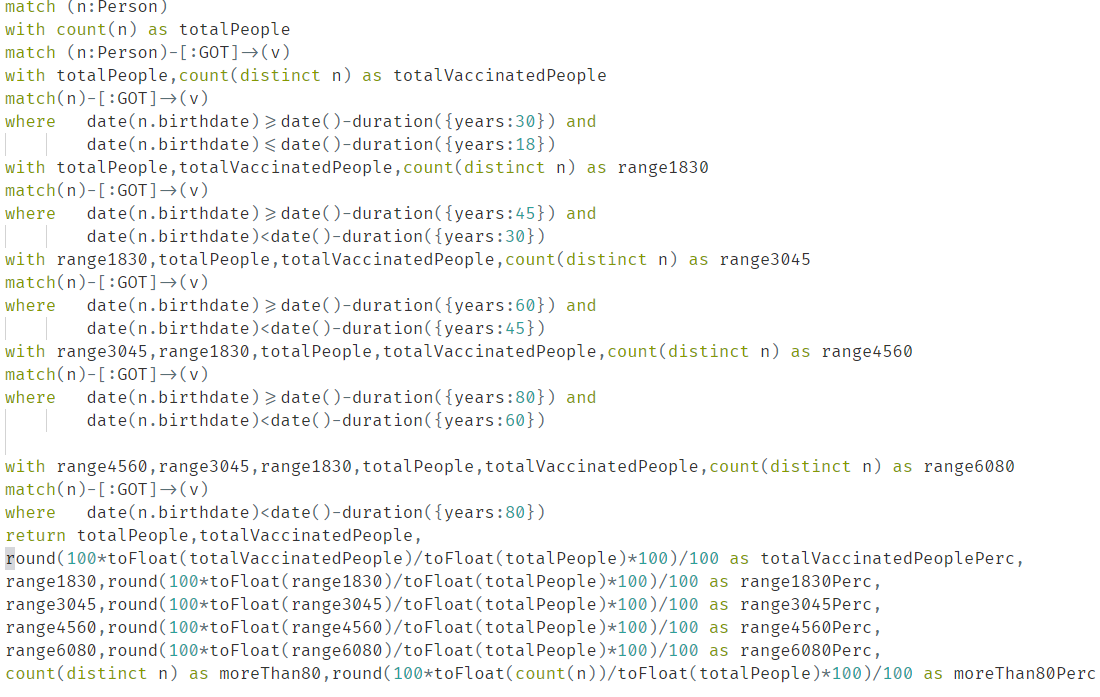
\includegraphics[width = 13 cm]{query5.png}}
\end{center}
\paragraph{} The output is given by: 
\begin{itemize}
\item[•] Total people
\item[•] Total vaccinated people (with \%)
\item[•] Vaccinated people in age ranges (with \%)
\begin{center}
	\fbox{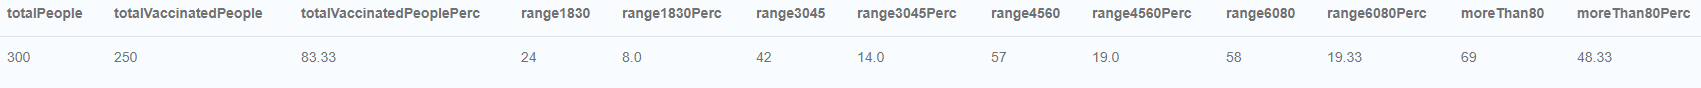
\includegraphics[width = 14 cm]{outputquery5.png}}
\end{center}
\end{itemize}

\subsection{Commands}
\subsubsection{Federico moves in an other house (CREATE)}
\paragraph{} In this command we simulate a person moving in an another house.
\begin{center}
	\fbox{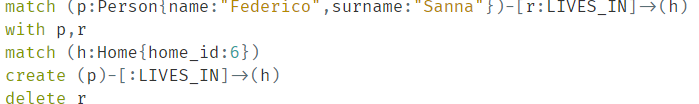
\includegraphics[width = 13 cm]{command1.png}}
\end{center}

\subsubsection{Delete all the public place records older than 1 year (DELETE) }
\paragraph{} In this command we simulate the need of removing old records that are not useful anymore.
\begin{center}
	\fbox{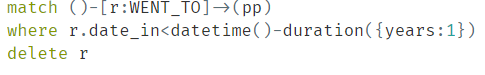
\includegraphics[width = 11 cm]{command2.png}}
\end{center}

\subsubsection{Name change of public place (UPDATE)}
\paragraph{} In this command we simulate the need, of a public place manager, of changing name of the activity.
\begin{center}
	\fbox{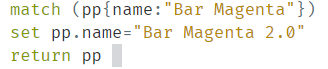
\includegraphics[width = 8 cm]{command3.png}}
\end{center}
\clearpage
\section{UI description \& User Guide}
\subsection{UI description}
\paragraph{}The design of the information system ended with the development of \emph{ContagionShield}, an application connected to the database with a simple GUI that is very intuitive and easy to use. The UI was created with the Python programming language by means of the libraries: \emph{PySimpleGUI} for the creation of the graphical interface, \emph{Py2neo} to work with Neo4j through the syntax offered by Python and \emph{pandas} to manage the analysis and manipulation of data, you can find these ones into the folder \texttt{"contagionshield"}. \par
	\begin{center}
 		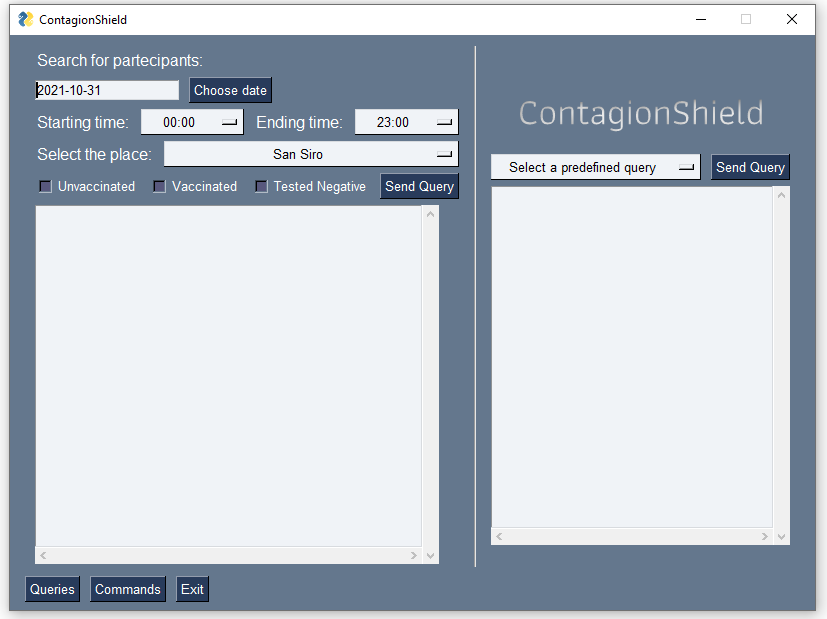
\includegraphics[width = 11 cm]{queriespage.PNG}
		\captionof{figure}{Query Interface}
	\end{center}
As you can see from \textbf{Figure 3}, the main screen of the application is divided into two sections: one on the left that allows you to create customizable queries by choosing date, place, time interval and whether to display the vaccinated, non-vaccinated or with negative test, in \textbf{Figure 4} there is an example query with the results obtained; the other side section on the right (\textbf{Figure 5}) presents some predefined queries, some of them follow the ones specified and described in Chapter 5 of the report. \par
	\begin{center}
 		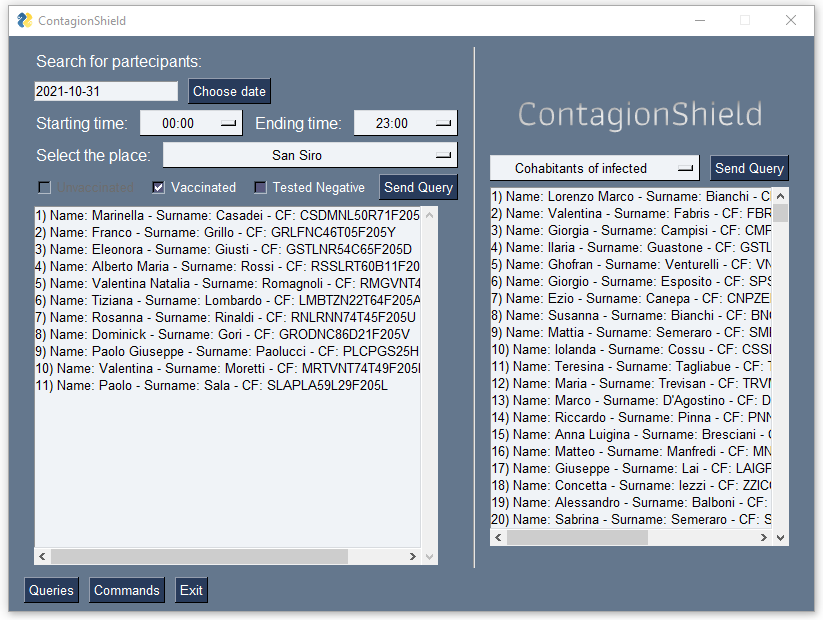
\includegraphics[width = 11 cm]{queriesresult.PNG}
		\captionof{figure}{Example Query with Results}
	\end{center}
	\begin{center}
 		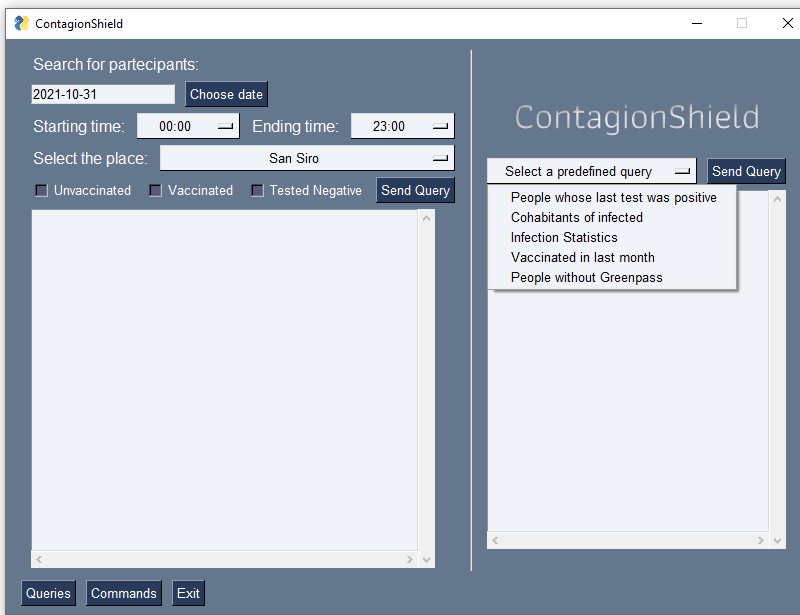
\includegraphics[width = 11 cm]{queriesexpanded.png}
		\captionof{figure}{Predefined Queries}
	\end{center}
\pagebreak
Finally, as shown in \textbf{Figure 6}, it is possible to execute some of the commands already presented in Chapter 5 by reaching the appropriate section of the application by means of the \texttt{"Commands"} button in the lower left corner of the main screen. The executable commands allow you to create new meetings between several people by indicating their social security numbers, the date and time, create new visits to public places by specifying who went to a given place and when and in the end you can also delete all the visits to public places recorded in the last year. \par
	\begin{center}
 		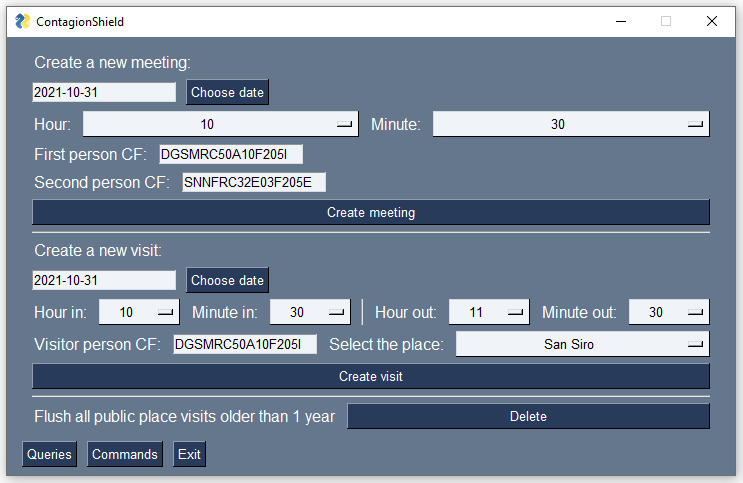
\includegraphics[width = 11 cm]{commandpage.PNG}
		\captionof{figure}{Command Interface}
	\end{center}
\subsection{User Guide}
\paragraph{}
In order to run \emph{ContagionShield} it is necessary to verify some requirements and to perform some actions:
\begin{itemize}[noitemsep]
   \item[-] At first you have to check if you have the right Python version installed by using the command: \texttt{python --version}, if not you could download it from the official website: https://www.python.org/ 
   \item[-] Then make sure your local database is at \texttt{localhost:7687} and that it has \texttt{"smbud"} as password
   \item[-] Install the required packages (in the "contagionshield" folder): \texttt{pip install -r requirements.txt}
   \item[-] Finally make it run by navigating to the folder where you have been saved the materials, then into \texttt{"contagionshield"} folder and run: \texttt{python contagionshield.py}
   \item[-] From there you can execute queries about the collected data
\end{itemize}
\newpage
\section{References \& Sources}
  \begin{thebibliography}{9}
    \bibitem{} Course Slides
    \bibitem{} https://pysimplegui.readthedocs.io/en/latest/call%20reference/
    \bibitem{} https://py2neo.org/
    \bibitem{} https://neo4j.com/docs/cypher-manual/current/
    \bibitem{} https://neo4j.com/developer/python/
    \bibitem{} http://iniball.altervista.org/Software/ProgER
    \bibitem{} https://neo4j.com/developer/cypher/
    \bibitem{} https://pandas.pydata.org/docs/
  \end{thebibliography}
\end{document}
